\section{RTOS Extension}

Many RTOS allow developers to create their own extensions that will be used by other developers to enhance and add functionnalities to their applications.
In these extensions, we can found modules that allow the use of FTP or COAP or even a Shell.
In the case of Contiki, those modules are called 'apps'.
To use those apps, the developer need to specify them in the \texttt{Makefile}.

\begin{lstlisting}[style=CStyle, language=make, caption=Example of Makefile using the app \texttt{shell} with Contiki]
CONTIKI_PROJECT = example
all: $(CONTIKI_PROJECT)

CONTIKI = ../contiki
APPS += shell # Using the shell app

include $(CONTIKI)/Makefile.include
\end{lstlisting}

For this second approach, we decided to develop our framework as a Contiki app.
The idea is to cause each task to ping the framework with its thread ID at the start and at the end of its execution.
In this way, the framework will keep track of which task is running and can detect a context switch and compute its duration.

\begin{figure}[!ht]
  \centering
  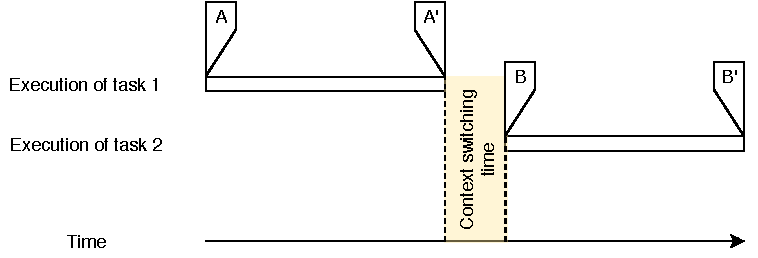
\includegraphics[scale=1]{assets/internal-framework-ping.pdf}
  \caption{\label{fig:internal-framework-ping}Pings to the framework}
\end{figure}

In the figure \ref{fig:internal-framework-ping}, we can see an example of usage with two tasks.
The task 1 pings the framework at steps A and A' with its thread ID of 1, respectively the start and the end of its execution.
The task 2 do the same at steps B and B' but with its thread ID of 2.
The context switch occurs between the steps A' and B and the framework can use the received pings to deduce the context switching time.

\subsection{Implementation}

\subsubsection{Framework implementation}
The implementation uses an internal structure \texttt{bench\_context} to store the last thread ID received with a ping and a timer to mesure the potential context switch.
Once a ping is received with the \texttt{bench\_ping(uint32\_t)} call, the framework store the new thread ID in its context and check if a change of thread IDs occurs with the \texttt{check\_change()} function.
If the two thread IDs match, no context switch happened and the same task is running on the foreground.
If the old thread ID does not match the new thread ID, it means a context switch just occur.
The context switching time is then computed using the timer stored in the context of the framework.
Finally, the time is reset.

The documented source code can be found in the listing \ref{lst:internal-bench-code}.

\begin{lstlisting}[float, style=CStyle, label={lst:internal-bench-code}, caption={Source code of the benchmarking framework implemented in Contiki}]
/**
  * Struct that stores benchmarking information.
  * 
  * previous_id: The id of the previous thread that performs a ping;
  * new_id: The id of the current thread that has performed a ping;
  * current_time: the timer
  */
struct BContext {
  uint32_t previous_id;
  uint32_t new_id;
  clock_time_t current_time;
} bench_context;


void bench_ping(uint32_t id) {
  // Save the new id
  bench_context.new_id = id;
  // Save the current time
  // Check for switching context
  if (!check_change()) {
    bench_context.current_time = RTIMER_NOW(); // Ticks
  }
}

int check_change(void) {
  if(bench_context.new_id != bench_context.previous_id) {
    // Compute the difference
    clock_time_t previous = bench_context.current_time;
    clock_time_t current = RTIMER_NOW();
    clock_time_t result = current - previous;

    // Keep the previous id for log
    uint32_t previous_id = bench_context.previous_id;
    // Change previous_id to new_id
    bench_context.previous_id = bench_context.new_id;

    bench_context.current_time = RTIMER_NOW(); // Ticks

    printf("[BENCH_CONTEXT_SWITCHING] %lu %lu %lu\n", previous_id, bench_context.new_id, result);
    
    return 1; // Change occurs
  }
  return 0; // No change
}
\end{lstlisting}

\subsubsection{Task implementation}

We wanted to make our benchmarking framework hidden for the developer.
But in order to compute the context switching time, our simple task has to be changed to call the \texttt{bench\_ping(uint32\_t)} of our framework.
The listing \ref{lst:bench-task-code} shows how we integrated our framework in the simple task.

\begin{lstlisting}[float, style=CStyle, label={lst:bench-task-code}, caption={Source code of the task with benchmarking framework calls}]
PROCESS_THREAD(task, ev, data)
{
    PROCESS_BEGIN();

    while (1)
    {
        PROCESS_PAUSE();
        bench_ping(TASK_ID); // Ping the framework
        // Wait for 1ms
        clock_delay_usec(1000);
        bench_ping(TASK_ID); // Ping the framework
    }

    PROCESS_END();
}
\end{lstlisting}